\documentclass[Report.tex]{subfiles}


\usepackage{graphicx}

\begin{document} 
\begin{figure}
	\center
	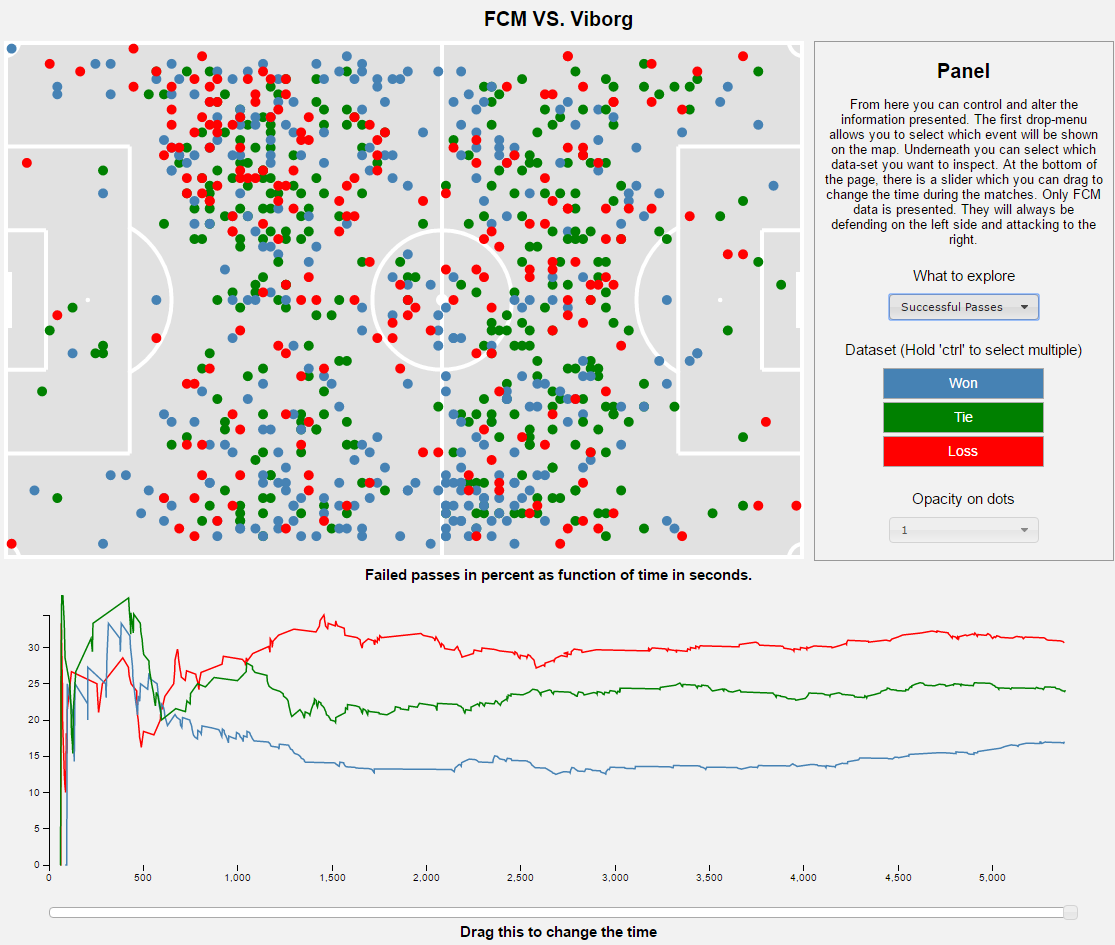
\includegraphics[width=\textwidth]{test.png}
	\caption{The successful passes on the map and the relationship between failed and successful ones in the line chart. Notice how a lot of passes happens over the middle while losing or playing tie. Interact with it live here.
	\label{Fig:}
\end{figure}


\subsubsection*{What-why-how}
The visualization attempts to give an overview of the three matches played between FCM and Viborg this season from FCM's point of view. The visualization presents various information regarding where touch-related data has taken place and also keeps track of the rate which different types of errors has occurred in percent.

The purpose is to allow the user to explore how a top-tier team such as FCM, deducted by the fact that they won the league in 2014/2015 and at the moment of writing is number three, can play against a new-coming underdog team from first division and in some cases win, play tie and lose. The hypothesizes is that their play-style will change when being behind, partly because they are not playing well in the first place, but also due to the pressure of losing to a on paper worse team.

To strengthen the hypothesis the visualization gives two different views where information can be deducted to find differences. The first one is a map which display where curtain events have taken place. The type of event is determined by the user in the selection-menu in the panel to the right. Six options are available and can be categorized into three overall themes which are: Aerial duals, shots and passings where for each the user can also select whether he wants to inspect the "successful" ones or the those that went wrong. By mapping the events, the user can look for clusters in the data and may find patterns to where curtain events happen. To aid in finding such clusters, two more options are available in the panel. The first one allows the user to select which matches should be inspected as the dots on the map may at time be so overwhelming that nothing can be concluded at all. Each match is represented by its own color with high variety in hue and brightness so they are easier to differentiate and also the background is very neutral to avoid interference with the inspected elements. The background also have the lines of a real football field to give a better feel of where on the field the events have happened. The last option in the panel allows the user to select an opacity of the dots. As all the coordinates have been altered in such a way that it looks like FCM is always playing on the left side of the field, many dots may at times overlap and thus making them slightly more transparent enables the user to spot overlaps. The altering of the coordinates, serves the purpose of creating a more intuitive view to spot cluster and thus the opacity serves an important part in the exploration. The second view is a line-chart which illustrates the relation between two variables as a percent on the y-axis and the time which has passed in seconds on the x-axis. The relation which is shown depends on the selection in the panel, so it may be how many percent of the passes failed, shots were missed or aerial duels lost. The number lines will also toggle to the selection of matches in the panel. However, the opacity can not be change here as it is not necessary to read the information successfully and would merely be a distraction. Lastly at the very bottom is a slider which determines which point in the three matches the user desires to inspect. The slider also contains ranges so snapshots of the match can be inspected in further detail.
\subsubsection*{Code}

As the visualization required information about the relationship between different variables, it was a necessity to pre-process the data to avoid computing too much in D3 and keeping it responsive, R was used to do the task. Firstly, the required columns were selected from the data-sheets from the API, more specifically all touches and shot in all three matches. The shots were then filtered to only be of the type necessary for the visualization, each time a successful event or unsuccessful one occurred, a counter was incremented and the relationship between were noted at each row, thus making it easier to plot in a line chart. Also, each row was noted with its field coordinate to also allow map-plotting in d3. However, instead of setting the literal coordinates for each event, everything was firstly mirrored so it looked like FCM was always playing from the left side and attack the right to make it easier to find patterns. All the data was exported into three csv-files each representing a match. At load time, the D3 scripts would load each dataset and store it in a variable to avoid anymore I/O-operation in terms of loading sheets, as it ruined responsibility. To alter the display, some global variables were responsible for how the filters worked and thus what data was included for display which were set by using the control panel. 

	
\end{document}